\documentclass[12pt]{article}
\usepackage[utf8]{inputenc}
\usepackage{mathtools}
\usepackage{graphicx}
\usepackage{subfig}
\usepackage{float}
\usepackage[export]{adjustbox}
\usepackage{amsmath}
\usepackage{listings}
\usepackage{color}

\graphicspath{{./report/}}

\definecolor{codegreen}{rgb}{0,0.6,0}
\definecolor{codegray}{rgb}{0.5,0.5,0.5}
\definecolor{codepurple}{rgb}{0.58,0,0.82}
\definecolor{backcolour}{rgb}{0.95,0.95,0.92}
 
\lstdefinestyle{mystyle}{
    backgroundcolor=\color{backcolour},   
    commentstyle=\color{codegreen},
    keywordstyle=\color{magenta},
    numberstyle=\tiny\color{codegray},
    stringstyle=\color{codepurple},
    basicstyle=\scriptsize,
    breakatwhitespace=false,         
    breaklines=true,                 
    captionpos=b,                    
    keepspaces=true,                 
    numbers=left,                    
    numbersep=5pt,                  
    showspaces=false,                
    showstringspaces=false,
    showtabs=false,                  
    tabsize=2
}
\lstset{style=mystyle}
\begin{document}
\title{CSC411 Project2}
\author{Yifei Ai}
\date{}
\maketitle
% ------------------------- Part 1 -------------------------
\section*{Part 1}
The dataset is a dictionary consisting of 9 training sets which are just number 0 to 9 and 9 test sets. Each training set is a matrix with $M\times 784$ which M represents the number of handwritten digit images in the dataset and each row is an array of size $1\times 784$ is the flatten array of handwritten digit image, which originally is $28\times 28$.

I randomly pick 10 images for each number, they all looks pretty good. At least I believe they are classified to the correct number.

% TODO: Include the image
% ------------------------- Part 2 -------------------------
\section*{Part 2}
Notice to make it convinient, I simply assume we already append the bias vector to Weight matrix
\begin{lstlisting}[language=Python]
    def layer_computation(x, W, b, act_func=lambda x: x):
        L = np.dot(W.T, x) + b
      	output = softmax(L)
      	return L, output

    def batch_layer_computation(X, W):
        """ X is an input matrix with size NxM, N is the number of input units, M is
        the number of training cases. W is a weight matrix already append bias vector 
        with size (N+1)xL, L is the number of output layers. Notice we need extra 
        one row for bias, so we should append another row vector [1, 1, 1, 1, ... ,1] 
        to X to do implement the function. """
        one_array = np.ones(X.shape[1])
        X = np.vstack((X, one_array))
        L1 = np.dot(W.T, X)
        Y = softmax(L1)
        return Y
\end{lstlisting}

% ------------------------- Part 3 -------------------------
\section*{Part 3}
Suppose X is a matrix with size $N\times M$, where N is the number of input layer, M is the number of training cases. Let W be a matrix be $N\times L$ where L is the number of units in hidden layer. Here L is 10. The output matrix Y has size of $L\times M$
\begin{align}
    % \frac{\partial \mathcal{L}_{CE}}{\partial y_k} &= \frac{-t_k}{y_k}\\
    % \mathcal{L}_{CE}(y, t) &= -t^T(logy)\\
    %                        &= -\sum_{j=1}^K t_j logy_j\\
    %                        &= -\sum_{j=1}^K t_j log\frac{e^{o_j}}{\sum_i e^{o_i}}\\
    %                        &= -\sum_{j=1}^K t_j (loge^{o_j} - log\sum_i e^{o_i})\\
    %                        &= -\sum_{j=1}^K t_j (o_j - log\sum_i e^{o_i})\\
    % \frac{\partial \mathcal{L}_{CE}}{\partial o_k} 
    % &= -t_k + \frac{e^{o_k}}{\sum_i e^{o_i}}\sum_{j=1}^K t_j && \text{Notice $\sum_{j=1}^K t_j = 1$}\\
    % &= -t_k + \frac{e^{o_k}}{\sum_i e^{o_i}}\\
    % &= -t_k + y_k\\
    % &= y_k - t_k
    y_j^{(i)} &= \frac{e^{o_j^{(i)}}}{\sum_k e^{o_k^{(i)}}}\\
    o_k^{(i)} &= \sum_{p=1}^{N}w_{pk}x_p^{(i)}+b_k\\
    \mathcal{L}_{CE} 
    &= \sum_{i=1}^M \sum_{j=0}^{L-1} -t_j^{(i)}logy_j^{(I)}\\
    &= \sum_{i=1}^M \sum_{j=0}^{L-1} -t_j^{(i)}[o_j^{(i)}-log(\sum_{k=0}^{L-1} e^{o_k^{(i)}})]\\
    &= \sum_{i=1}^M \sum_{j=0}^{L-1} -t_j^{(i)}[\sum_{p=1}^{N}w_{pj}x_p^{(i)}+b_j - log\sum_k (e^{\sum_{p=1}^{N}w_{pk}x_p^{(i)}+b_k})]\\
    \frac{\partial \mathcal{L}_{CE}}{\partial w_{sm}}
    &= \sum_{i=1}^M [(-t_m^{(i)} + \frac{e^{\sum_{s=1}^{N}w_{sm}x_s^{(i)}+b_m}}{\sum_k (e^{\sum_{p=1}^{N}w_{pk}x_p^{(i)}+b_k})}\sum_{j=0}^{L-1} t_j^{(i)})\,\,x_s^{(i)}]\\ \text{Notice $\sum_{j=1}^{L-1} t_j = 1$}\\
    &= \sum_{i=1}^M [(-t_m^{(i)} + \frac{e^{o_m^{(i)}}}{\sum_k e^{o_k^{(i)}}})x_s^{(i)}]\\
    &= \sum_{i=1}^M [(-t_m^{(i)} + y_m^{(i)})x_s^{(i)}]
\end{align}
Therefore, we get the derivative of weight is:
\[
    \frac{\partial \mathcal{L}_{CE}}{\partial W} = X(Y-T)^T
\]
To approximate the gradient, I use the following code:
\begin{lstlisting}[language=Python]
    def approx_CE_dWeight_single(X, W, T, p, q, t):
        """Approximate the derivative of single entry in Jacobian matrix"""
        new_weight = W.copy()
        new_weight[p][q] += t
        Y = batch_layer_computation(X, W)
        Y_h = batch_layer_computation(X, new_weight)
        df = part3_cross_entropy(Y_h, T) - part3_cross_entropy(Y, T)
        df = np.true_divide(df, t)
        return df

    def approx_CE_dWeight(X, W, T, t=1e-4):
        size = W.shape
        df_matrix = np.empty(size, dtype=np.float64)
        for i in range(size[0]):
            for j in range(size[1]):
                df_matrix[i][j] = approx_CE_dWeight_single(X, W, T, i, j, t)
        return df_matrix
\end{lstlisting}
I wrote some test case to test the function. Notice here W already append the bias vectors.
\begin{lstlisting}
In [130]: X
Out[130]: 
array([[1, 5],
       [2, 4]])

In [131]: W
Out[131]: 
array([[3., 4., 7.],
       [2., 5., 9.],
       [3., 2., 6.]])

In [143]: Y = ast2.batch_layer_computation(X, W)

In [144]: Y
Out[144]: 
array([[7.58255810e-10, 7.09547416e-23],
       [3.05902227e-07, 6.30511676e-16],
       [9.99999693e-01, 1.00000000e+00]])

In [133]: T
Out[133]: 
array([[1, 0],
       [0, 1],
       [0, 0]])

In [134]: ast2.CE_dWeight(X, Y, T)
Out[134]: 
array([[-1.        , -4.99999969,  5.99999969],
       [-2.        , -3.99999939,  5.99999939],
       [-1.        , -0.99999969,  1.99999969]])


In [135]: ast2.approx_CE_dWeight(ast2.batch_layer_computation, X, W, T)
Out[135]: 
array([[-1.        , -4.99999969,  5.99999969],
       [-2.        , -3.99999939,  5.99999939],
       [-1.        , -0.99999969,  1.99999969]])

In [184]: X
Out[184]: 
array([[2, 8],
       [1, 9]])

In [185]: W
Out[185]: 
array([[1., 7., 2.],
       [0., 7., 5.],
       [6., 8., 4.]])

In [186]: Y = ast2.batch_layer_computation(X, W)

In [187]: Y
Out[187]: 
array([[7.58255957e-10, 8.40859712e-50],
       [9.99999887e-01, 1.00000000e+00],
       [1.12535162e-07, 1.18506486e-27]])

In [188]: ast2.CE_dWeight(X, Y, T)
Out[188]: 
array([[-2.00000000e+00,  1.99999977e+00,  2.25070324e-07],
       [-9.99999999e-01,  9.99999887e-01,  1.12535162e-07],
       [-9.99999999e-01,  9.99999887e-01,  1.12535162e-07]])

In [189]: ast2.approx_CE_dWeight(X, W, T)
Out[189]: 
array([[-2.00000000e+00,  1.99999977e+00,  2.25099939e-07],
       [-9.99999999e-01,  9.99999887e-01,  1.12549969e-07],
       [-9.99999999e-01,  9.99999887e-01,  1.12549969e-07]])
\end{lstlisting}

% ------------------------- Part 4 -------------------------

% ------------------------- Part 5 -------------------------
\section*{Part 5}
I just simply follow the algorithm, momentum is at line 29
\begin{lstlisting}[language=Python]
def gradient_descent(X, T, alpha=0.00001, EPS = 1e-5, max_iter = 300, mu = 0):
    """ X is the matrix of inputs, NxM, N is the number of input units, M is the 
    number of training cases. T is the matrix of results, size: LxM, L is the 
    number of output units """
    # Initialize a weight matrix
    size = [X.shape[0], T.shape[0]]
    print "Weight size is:" + str(size)
    W = initialize_weights(size)
    b = initialize_bias(T.shape[0])
    previous_W = W - 10*EPS
    previous_b = b - 10*EPS
    count = 0
    perform_dict = dict()

    summary = np.empty((6, 0), dtype=float)

    X_test, T_test, X_valid, T_valid = seperate_train_valid()

    p = 0
    
    while norm(W - previous_W)+norm(b - previous_b) > EPS and count < max_iter:
        previous_W = W.copy()
        b = b.copy()
        Y = batch_layer_computation(X, W, b)
        Y_test = batch_layer_computation(X_test, W, b)
        Y_valid = batch_layer_computation(X_valid, W, b)
        data = calculate_data(Y, T, Y_test, T_test, Y_valid, T_valid)
        summary = np.hstack((summary, data[:,None]))
        p = mu*p + alpha*CE_dWeight(X, Y, T)
        W = W - p
        b = b - alpha*CE_dBias(Y, T)
        print "Iter: " , count
        print "Weight: " , W
        print "Cost: " , part3_cross_entropy(Y, T)
        if count % (max_iter/5) == 0:
            print "Accuracy on test set: ", calculate_accuracy(Y, T)
            perform_dict[count] = (calculate_accuracy(Y, T), previous_W, previous_b)
        count += 1
    if mu == 0:
        np.save('tmp/part4_summary_data'+str(alpha), summary)
    else:
        np.save('tmp/part4_summary_data_momentum'+str(alpha), summary)
    return W, b, perform_dict
\end{lstlisting}
We can see that gradient descent with momentum converge much faster than the one without using momentum
\begin{figure}[h]
    \subfloat[label 1]{{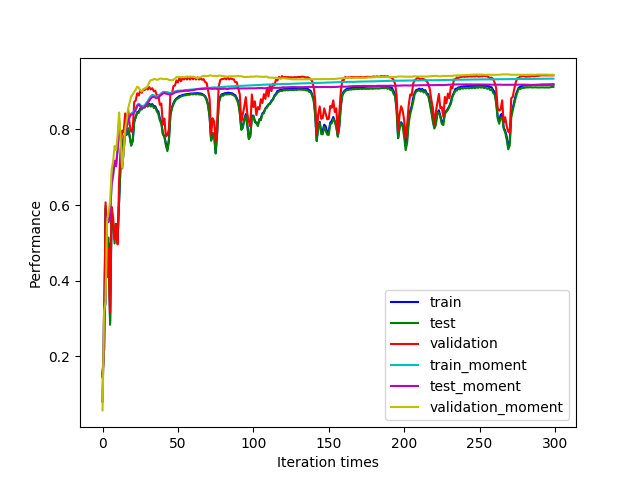
\includegraphics[width=0.5\textwidth]{./report/part5_300iter_5e-5_performance.png}}}
    \qquad
    \subfloat[label 2]{{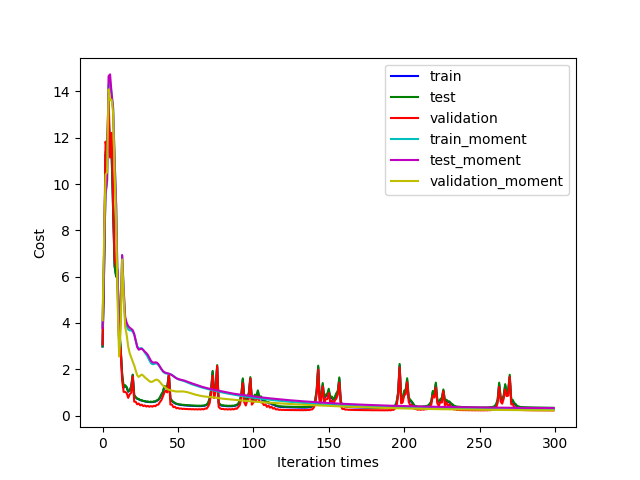
\includegraphics[width=0.5\textwidth]{./report/part5_300iter_5e-5_cost.png}}}
    \caption{Learning rate $5\times 10^{-5}$}
\end{figure}
\begin{figure}[H]
    \subfloat[label 1]{{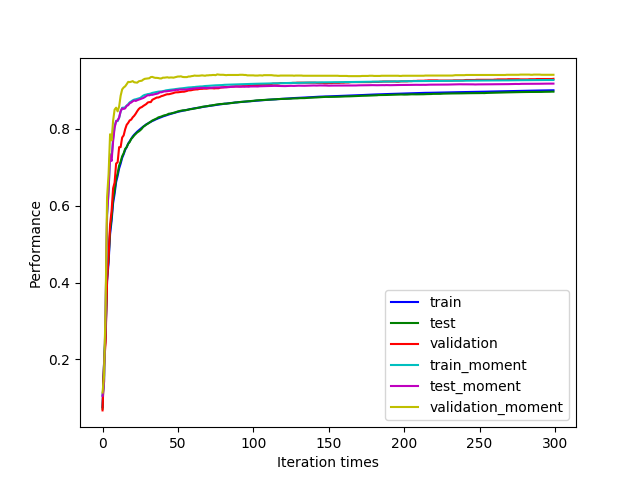
\includegraphics[width=0.5\textwidth]{./report/part5_300iter_1e-5_performance.png}}}
    \qquad
    \subfloat[label 2]{{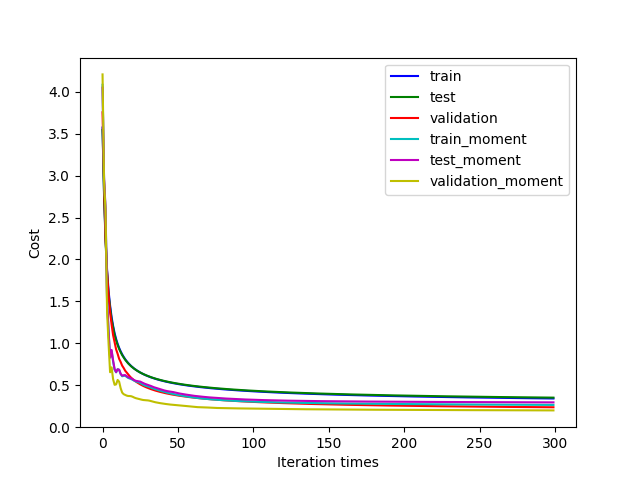
\includegraphics[width=0.5\textwidth]{./report/part5_300iter_1e-5_cost.png}}}
    \caption{Learning rate $1\times 10^{-5}$}
\end{figure}

% ------------------------- Part 6 -------------------------
\section*{Part 6}
\subsection*{(a)}
\begin{figure}[h]
    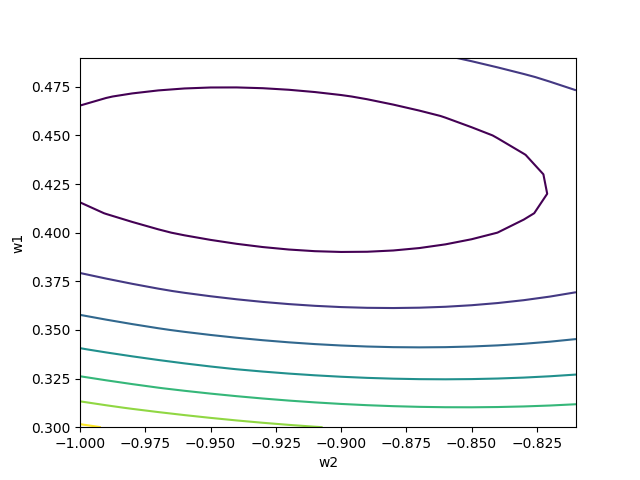
\includegraphics[width=0.5\textwidth]{./report/part6a_contour.png}
    \caption{Contour set with w1 and w2 around optimum}
\end{figure}

\subsection*{(b), (c)}
I tried several examples, these two demonstrate the feature of momentum
\begin{figure}[H]
    \subfloat[label 1]{{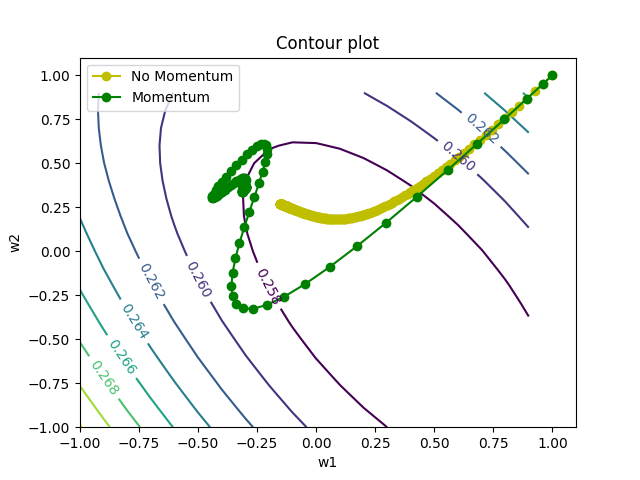
\includegraphics[width=0.5\textwidth]{./report/part6bc_nice.png}}}
    \qquad
    \subfloat[label 2]{{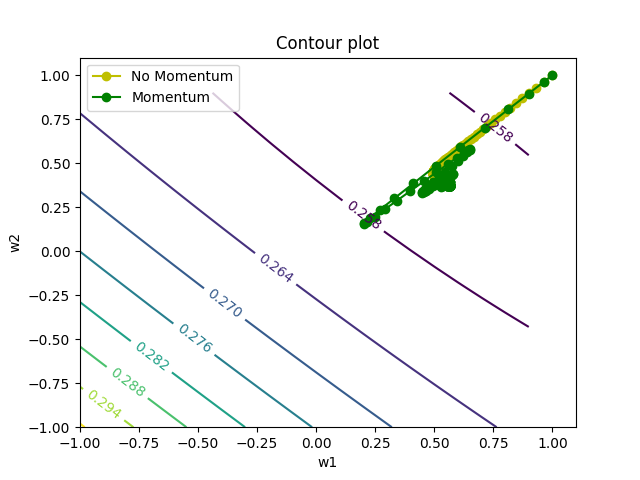
\includegraphics[width=0.5\textwidth]{./report/part6bc_nice2.png}}}
    \caption{trajectory for gradient descent with moment and without momentum}
\end{figure}

\subsection*{(d)}
The trajectory with momentum goes to the optimum faster, but would get around the optimum in a very small range compare with the trajectory without momentum. This is because we have momentum, that somehow remembers the direction of last update.

\subsection*{(e)}
We should choose the pixel in the center of the image. Our image is 28*28, so if we choose some variable on the edge then either the gradient descent on those 2 variables stop on first several steps or have a very slow trajectory. I think this is becuase it is on the edge, so since other entries in W is already close to optimum, so the variable on the edge doesn't really affect the result, in other word, it probably because the input is 0 corresponds to that entry is 0, so it doesn't really affect too much.

\begin{figure}[H]
    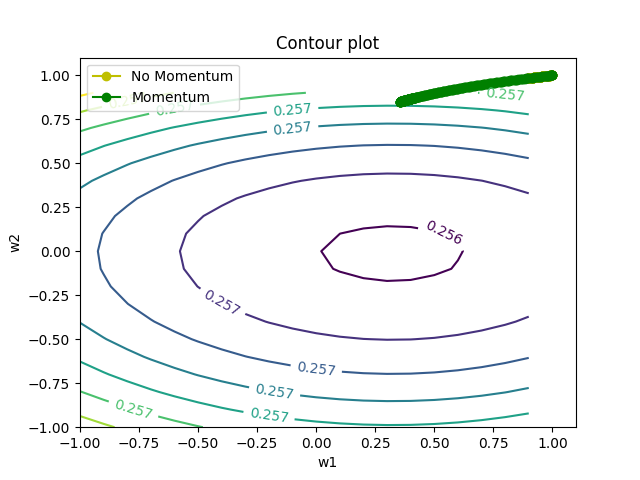
\includegraphics[width=\textwidth]{./report/partbc_contour_bad.png}
    \caption{trajectory that doens't demonstrate the benefit of momentum}
\end{figure}

This is the w1, w2 from W[100][8] and W[200][8], if we check the train set $M['train8'][i][100]$ and $['train8'][i][200]$, most of them are 0. We can see that 2 trajectories are almost the same.

To get a nice example, I simply look for some entry in M['train8'][i] that is not 0, since 8 relatively has more entries be gray compare with other number in my opinion. Then I do the gradient descent to those 2 variables on the W.

% ------------------------- Part 7 -------------------------
\section*{Part 7}
Suppose we use back propagation, then, denote $T(N)$ as the complexity with N layers.
\begin{figure}[h]
    \centering
    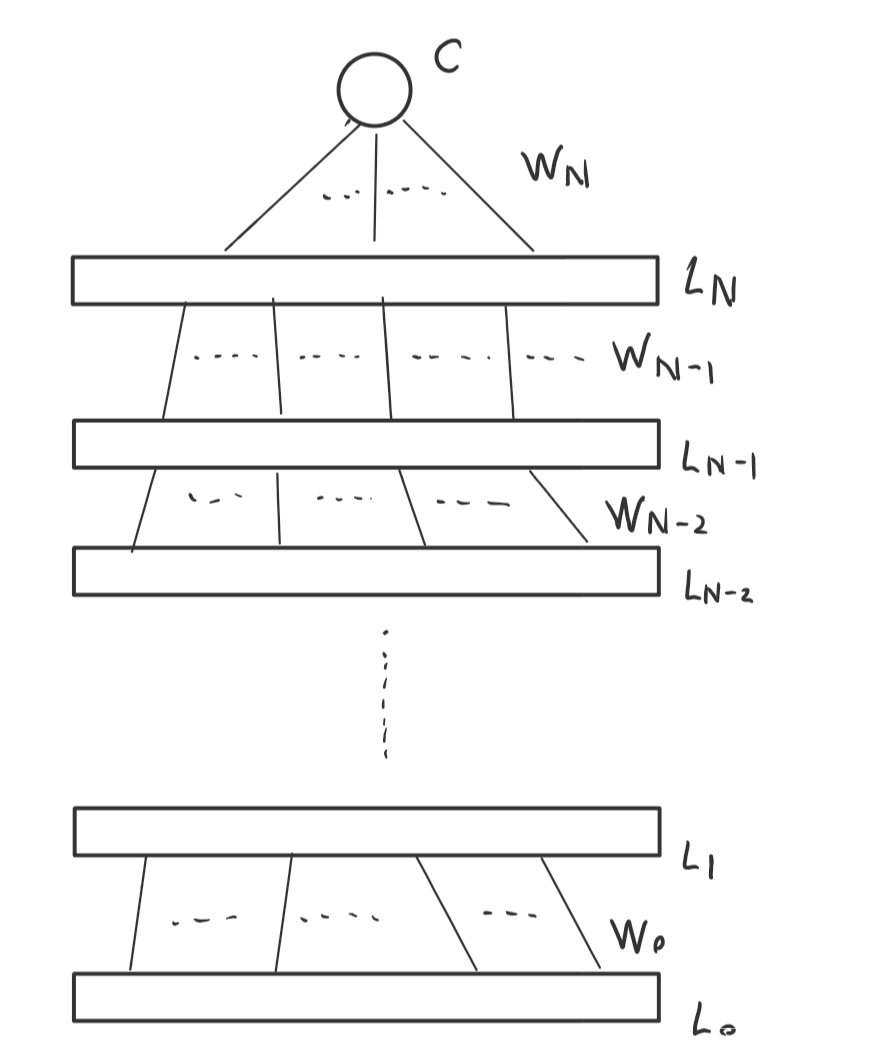
\includegraphics[scale=0.2]{report/part7_layer.jpg}
    \caption{Network with N+1 Layer}
\end{figure}
\subsection*{With Back Propagation}
Consider we have $N+1$ layers, now, if we need to calculate the gradients for all weights, then the first N layer we have calculate actually costs $T(N)$ by our assumption, then for the last layer, we need to know $\frac{\partial C}{\partial W_0}$. Since we use back propagation, we have $\frac{\partial C}{\partial L_2}$, thus we just need to calculate $\frac{\partial L_2}{\partial L_1}$ and $\frac{\partial L_1}{\partial W_0}$. So we will have
\[
    T(N+1) = T(N) + 2
\]
Which means complexity with back propagation is $O(N)$.
\subsection*{Without Back Propagation}
In this case, since we don't store any information, to calculate $\frac{\partial C}{\partial W_0}$, we need to do $\frac{\partial C}{\partial L_N}\frac{\partial L_N}{\partial L_{N-1}}\cdots \frac{\partial L_2}{\partial L_1}\frac{\partial L_1}{\partial W_0}$. So we will have
\[
    T(N+1) = T(N) + (N + 1)
\]
This means the complexity without back propagation is $O(N^2)$

% ------------------------- Part 8 -------------------------
\section*{Part 8}
I use a network with 32*32 or 64*64 input units, 6 output units, and one hidden layer. In that hidden layer, there are 12 hidden units, the activate function is ReLU. I tried both 32x32 and 64x64 to train the network, and I found the 32x32 has better performance. I guess the reason is 64x64 resolution cause overfitting. Also, learning rate with $10^{-4}$ has best performance on test set. Here are the final performance for each learning rate.
\begin{lstlisting}
Resolution: 32x32, doing gradient descent with learning rate: 0.01 ......
0.758333333333
Resolution: 32x32, doing gradient descent with learning rate: 0.001 ......
0.783333333333
Resolution: 32x32, doing gradient descent with learning rate: 0.0001 ......
0.791666666667
Resolution: 64x64, doing gradient descent with learning rate: 0.0001 ......
0.641666666667
Resolution: 64x64, doing gradient descent with learning rate: 1e-05 ......
0.725
Resolution: 64x64, doing gradient descent with learning rate: 1e-06 ......
0.525
\end{lstlisting}
\begin{figure}[h]
    \subfloat[rate 0.01]{{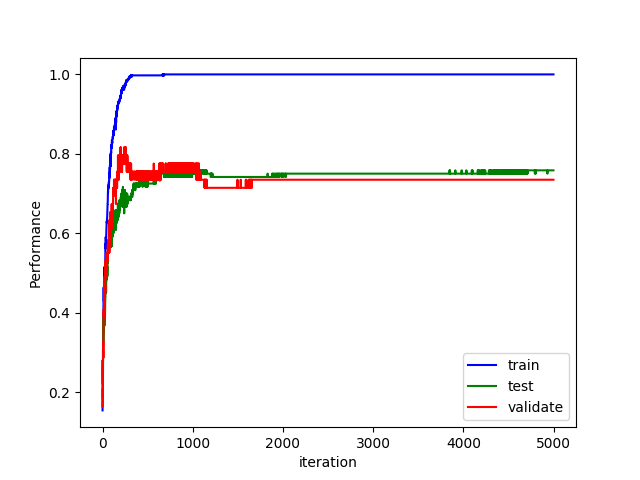
\includegraphics[width=0.28\textwidth]{report/part8_curves_performance1.png}}}
    \qquad
    \subfloat[rate 0.001]{{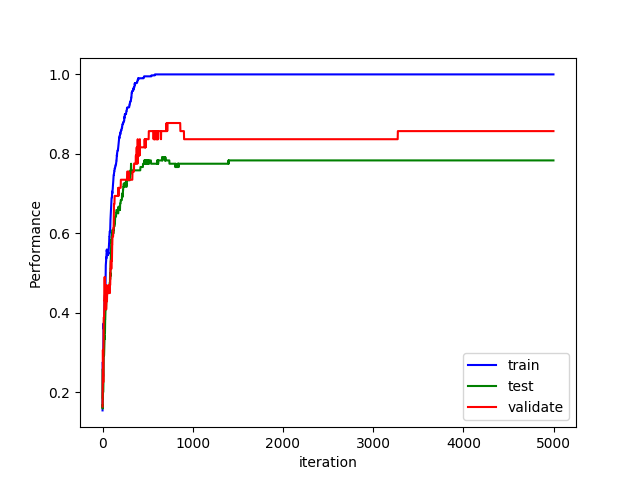
\includegraphics[width=0.28\textwidth]{report/part8_curves_performance2.png}}}
    \qquad
    \subfloat[rate 0.0001]{{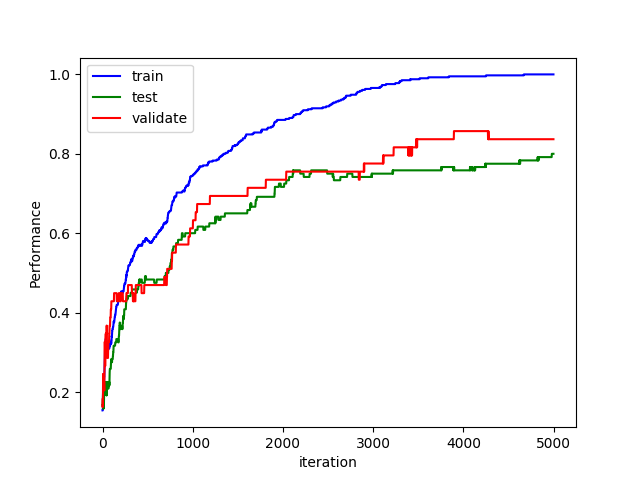
\includegraphics[width=0.28\textwidth]{report/part8_curves_performance3.png}}}
    \caption{Resolution 32x32, learning curve with rate 0.01, 0.001, 0.0001}
\end{figure}
\begin{figure}[h]
    \subfloat[rate 0.01]{{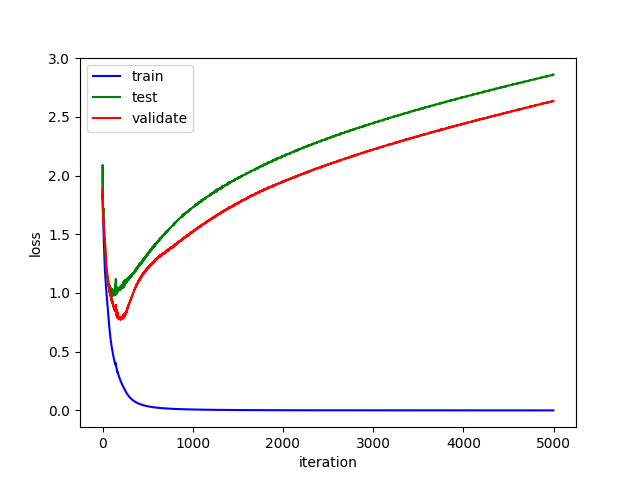
\includegraphics[width=0.28\textwidth]{report/part8_curves_loss1.png}}}
    \qquad
    \subfloat[rate 0.001]{{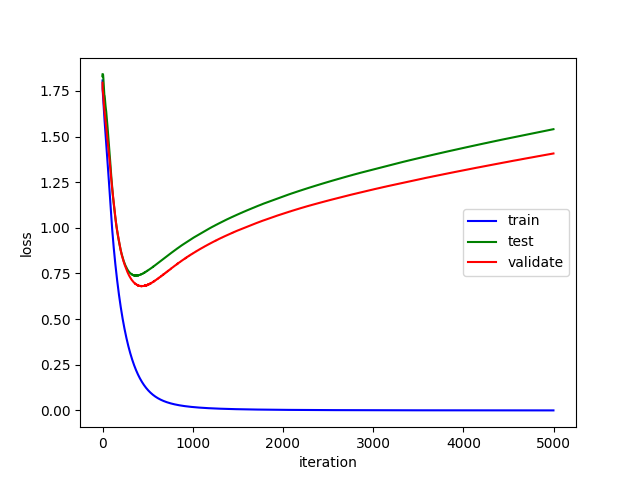
\includegraphics[width=0.28\textwidth]{report/part8_curves_loss2.png}}}
    \qquad
    \subfloat[rate 0.0001]{{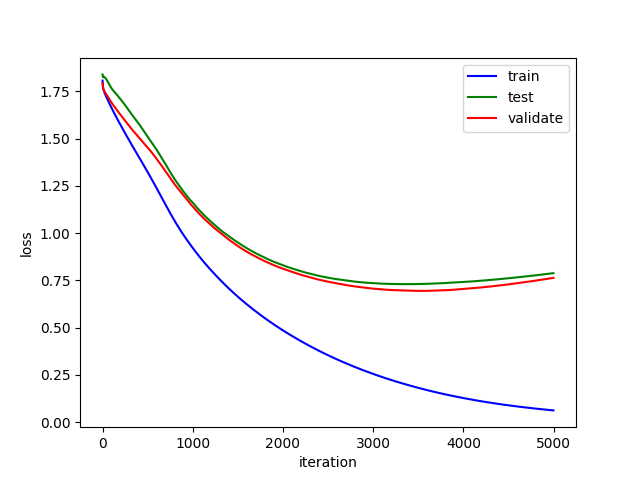
\includegraphics[width=0.28\textwidth]{report/part8_curves_loss3.png}}}
    \caption{Resolution 32x32, learning curve with rate 0.01, 0.001, 0.0001}
\end{figure}
\begin{figure}[h]
    \subfloat[rate 0.0001]{{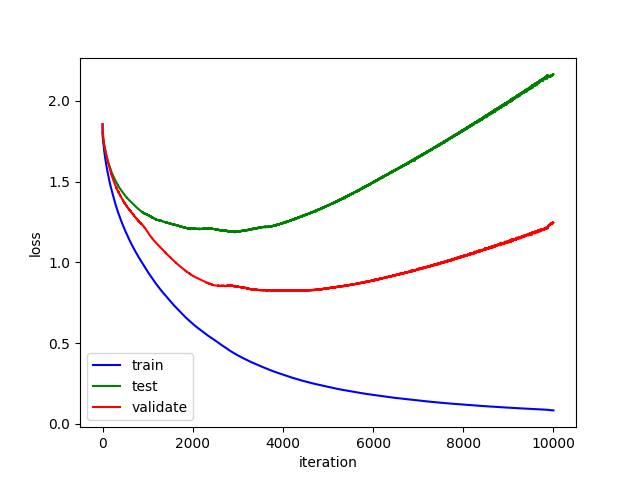
\includegraphics[width=0.28\textwidth]{report/part8_64curves_loss1.png}}}
    \qquad
    \subfloat[rate $10^{-5}$]{{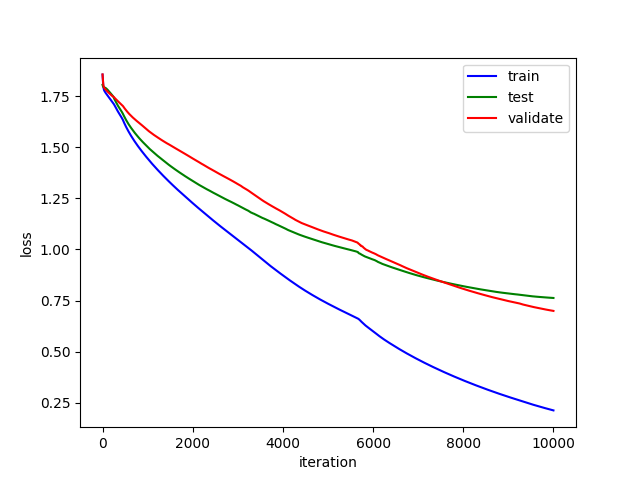
\includegraphics[width=0.28\textwidth]{report/part8_64curves_loss2.png}}}
    \qquad
    \subfloat[rate $10^{-6}$]{{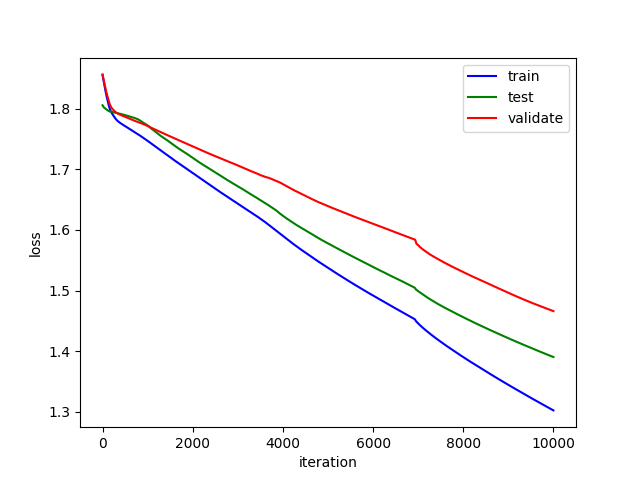
\includegraphics[width=0.28\textwidth]{report/part8_64curves_loss3.png}}}
    \caption{Resolution 64x64, learning curve with rate $10^{-4},10^{-5},10^{-6}$}
\end{figure}
\begin{figure}[H]
    \subfloat[rate 0.0001]{{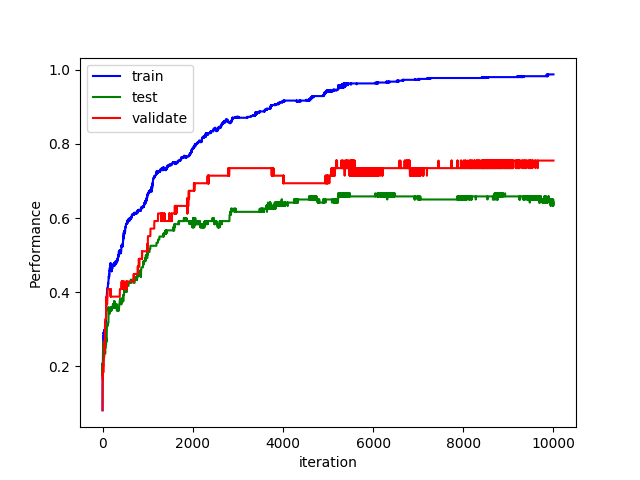
\includegraphics[width=0.28\textwidth]{report/part8_64curves_performance1.png}}}
    \qquad
    \subfloat[rate $10^{-5}$]{{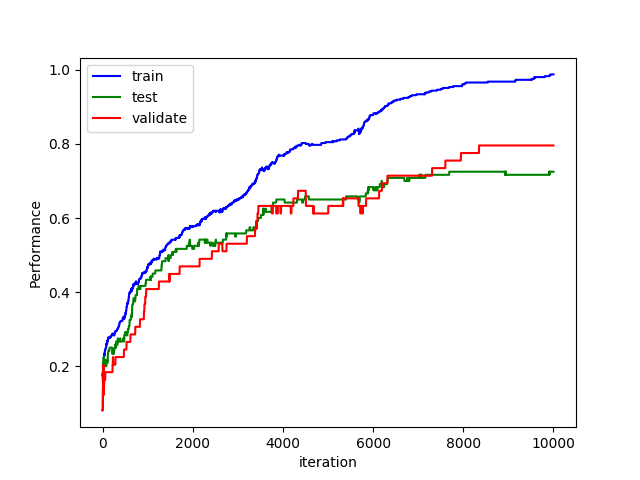
\includegraphics[width=0.28\textwidth]{report/part8_64curves_performance2.png}}}
    \qquad
    \subfloat[rate $10^{-6}$]{{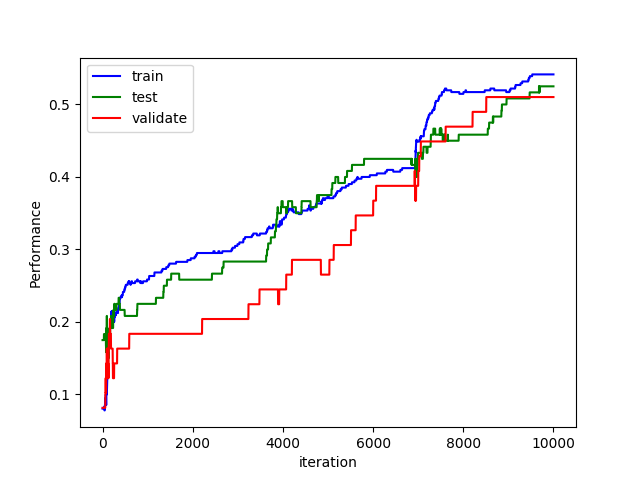
\includegraphics[width=0.28\textwidth]{report/part8_64curves_performance3.png}}}
    \caption{Resolution 64x64, learning curve with rate $10^{-4},10^{-5},10^{-6}$}
\end{figure}
\end{document}